\chapter{Data Analysis}

\MyQuote{In physics, you don't have to go around making trouble for yourself - nature
does it for you.}{Frank Wilczek}

QCD jets are the most common hard objects observed at hadron colliders, with
their cross section exceeding any other physics process by orders of magnitude.
Measurement of inclusive jet cross section thus provide the first test for both
QCD predictions and the detector performance. LHC Run II should open new
kinematic region with expectation of observation of jets with $\pt$ in $\TeV$
region.

This chapter describes the details of the inclusive jet cross section analysis.

\section{Data Characteristics}

Data used in this thesis are Monte Carlo generated events of $pp$ collisions at
the center-of-mass energy $\sqrt{s} = 13\TeV$ by \textsc{Pythia8}
(?citace?) event generator using CT10 PDFs (?citace?) and ATLAS underlying event
tune AU2 (?citace?). \textsc{Pythia8} performs LO QCD calculations. The response of
the ATLAS detector on these events was calculated with ?\textsc{Geant4}?
(?citace?) software toolkit.

Particles were recombined using anti-$k_t$ jet algorithm with parameter $R=0.4$.
There are parton jets reconstructed from the \textsc{Pythia8} output, which
further in this thesis are denoted truth jets, and next to them, there are the
signal jets reconstructed from the output of \textsc{Geant4} detector
simulation as the topological cell clusters. 

Generated events are divided into JZXW samples according to
the leading truth jet $\pt$. These samples differ in event weight which is for
the whole event calculated as the product of cross section, filter efficiency,
inverse number of events and additional weight factor which is for each event
stored in \texttt{EventInfoAux} container. Values used in this thesis are given
in Table \ref{tab:JZXW}.  

\begin{table}
  \centering
  \begin{tabular}{|c|rcr|c|c|c|}
    \hline 
     JZXW & \multicolumn{3}{|c|}{$\pt$ range (GeV)} & Cross-section (fb) & Filter Efficiency & \# envents  \\ 
    \hline
    \hline
		 JZ0W &     0 & - &    20 & 7.8420e+13 & 9.7193e-01 & 3498000 \\ 
    \hline
		 JZ1W &    20 & - &    80 & 7.8420e+13 & 2.7903e-04 & 2998000 \\
    \hline
		 JZ2W &    80 & - &   200 & 5.7312e+10 & 5.2261e-03 & 500000  \\
    \hline
		 JZ3W &   200 & - &   500 & 1.4478e+09 & 1.8068e-03 & 499500  \\
    \hline
		 JZ4W &   500 & - &  1000 & 2.3093e+07 & 1.3276e-03 & 477000  \\
    \hline
		 JZ5W &  1000 & - &  1500 & 2.3793e+05 & 5.0449e-03 & 499000  \\
    \hline
		 JZ6W &  1500 & - &  2000 & 5.4279e+03 & 1.3886e-02 & 493500  \\
    \hline
		 JZ7W &  2000 & + &       & 9.4172e+02 & 6.7141e-02 & 497000  \\
    \hline 
  \end{tabular}
  \caption{The cross-sections, filter efficiency and number of events for the JZXW samples which differ in the leading truth jet $\pt$.}
  \label{tab:JZXW}
\end{table}

Analysis uses jets with transverse momentum $\pt > 15\GeV$ and rapidity $|y| <
4$ and is done in $\pt$ and $|y|$ bins with the following edges

\small
\begin{align}
  \pt = \, &15:20:25:35:45:55:70:85:100:116:134:152:172:194:216:240:264:290: \nonumber \\
        &318:346:376:408:442:478:516:556:598:642:688:736:786:838:894:952: \nonumber \\
        &1012:1076:1162:1310:1530:1992:2300:2800:3400:4100:5000:6000:7200 \GeV \nonumber \\
  |y| = \, &0.0:0.5:1.0:1.5:2.0:2.5:3.0:3.5:4.0
  \label{eq:Binning}
\end{align}
\normalsize

\section{Event Selection}

Signal jets were calibrated using \textsc{ApplyJetCalibration} library version
3.28 and configuration parameters were loaded from the
\texttt{JES\_Full2012dataset\_May2014.config} with calibration sequence
\texttt{JetArea\_Residual\_EtaJES}. In next signal jets denotes the signal
calibrated jets.

In this section the jet selection criteria and matching of truth with signal
jets are described. The former is needed to cut those jets off, which were
misinterpreted by the detector, by the later the inputs for the unfolding
procedure are obtained. Description of the unfolding procedure will follow in
the next section.

\subsection{Jet Cuts}

\begin{itemize}
  \item \textbf{$\mathbf{\pt}$ Cut}

    something something something
  \item \textbf{$\mathbf{y}$ Cut}
    
    something something something
  \item \textbf{Zero jet (0jet) Cut}

    something something something
  \item \textbf{Leading Ration (LR) Cut}

    something something something
\end{itemize}

Discuss results of cutting. 
Figure \ref{fig:Cutting}
Table \ref{tab:CutAndMatchingEfficiency}

\subsection{Jet Matching}

Describe matching procedure.  
Discuss results of matching.
matchedSignal, unmatchedSignal, matchedTruth, unmatchedTruth.
Figure \ref{fig:Matching}
Table \ref{tab:CutAndMatchingEfficiency}


\section{Unfolding}

The main ingredient for the unfolding procedure is the transfer matrix Aij,
which is derived from Monte Carlo and contains the number of jets that have been
reconstructed in bin i with a matched truth jet that was generated in bin j. A
reconstructed and true jet are considered matched if their centers lie within
DeltaR <0.3 of each other, and the matching is unique. The transfer matrix does not
include unmatched jets, so an equivalent fraction of jets in data needs to be
removed from the unfolding procedure: a multiplicative inefficiency equal to the
fraction of unmatched jets is applied to data before the start of the unfolding
procedure, and the equivalent number of jets is restored after the unfolding.

How the unfolding matrix is filled.
MatchingEfficiency for signal and truth jets.
IDSUnfolding 

The unfolding procedure for the inclusive jet measurement is iterated once.


\begin{figure}[h]
  \centering
  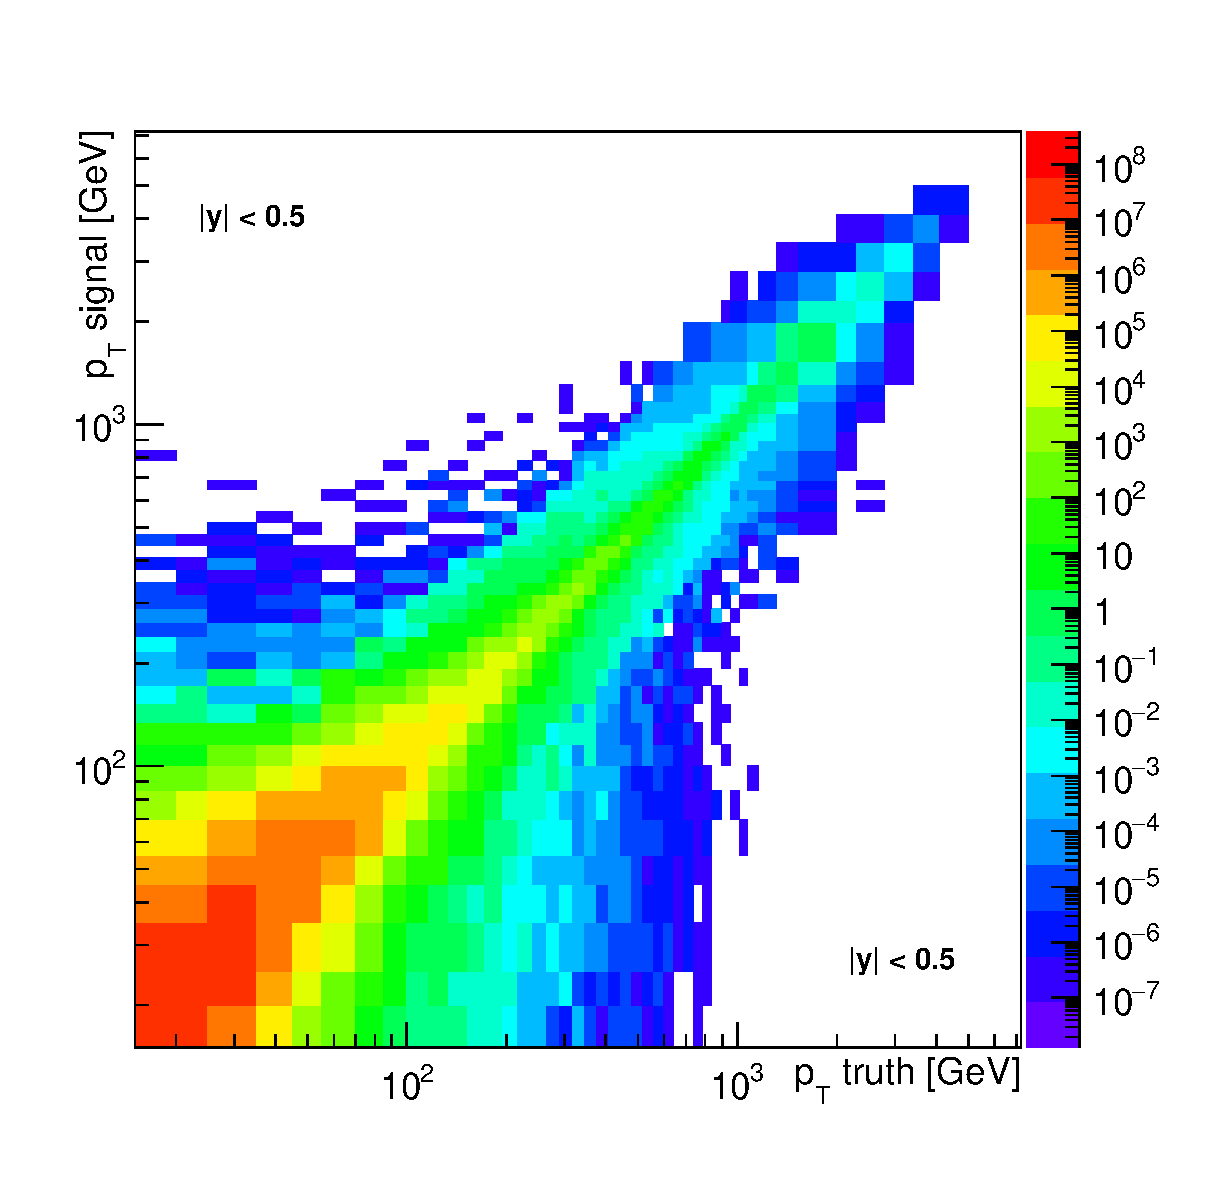
\includegraphics[width=0.7\textwidth]{{Chapter3/Unfold_matrix_firstBin}.eps}
  \caption{Unfolding matrix detail}
  \label{fig:UnfoldingMatrixDetail}
\end{figure}

\begin{figure}[h]
  \centering
  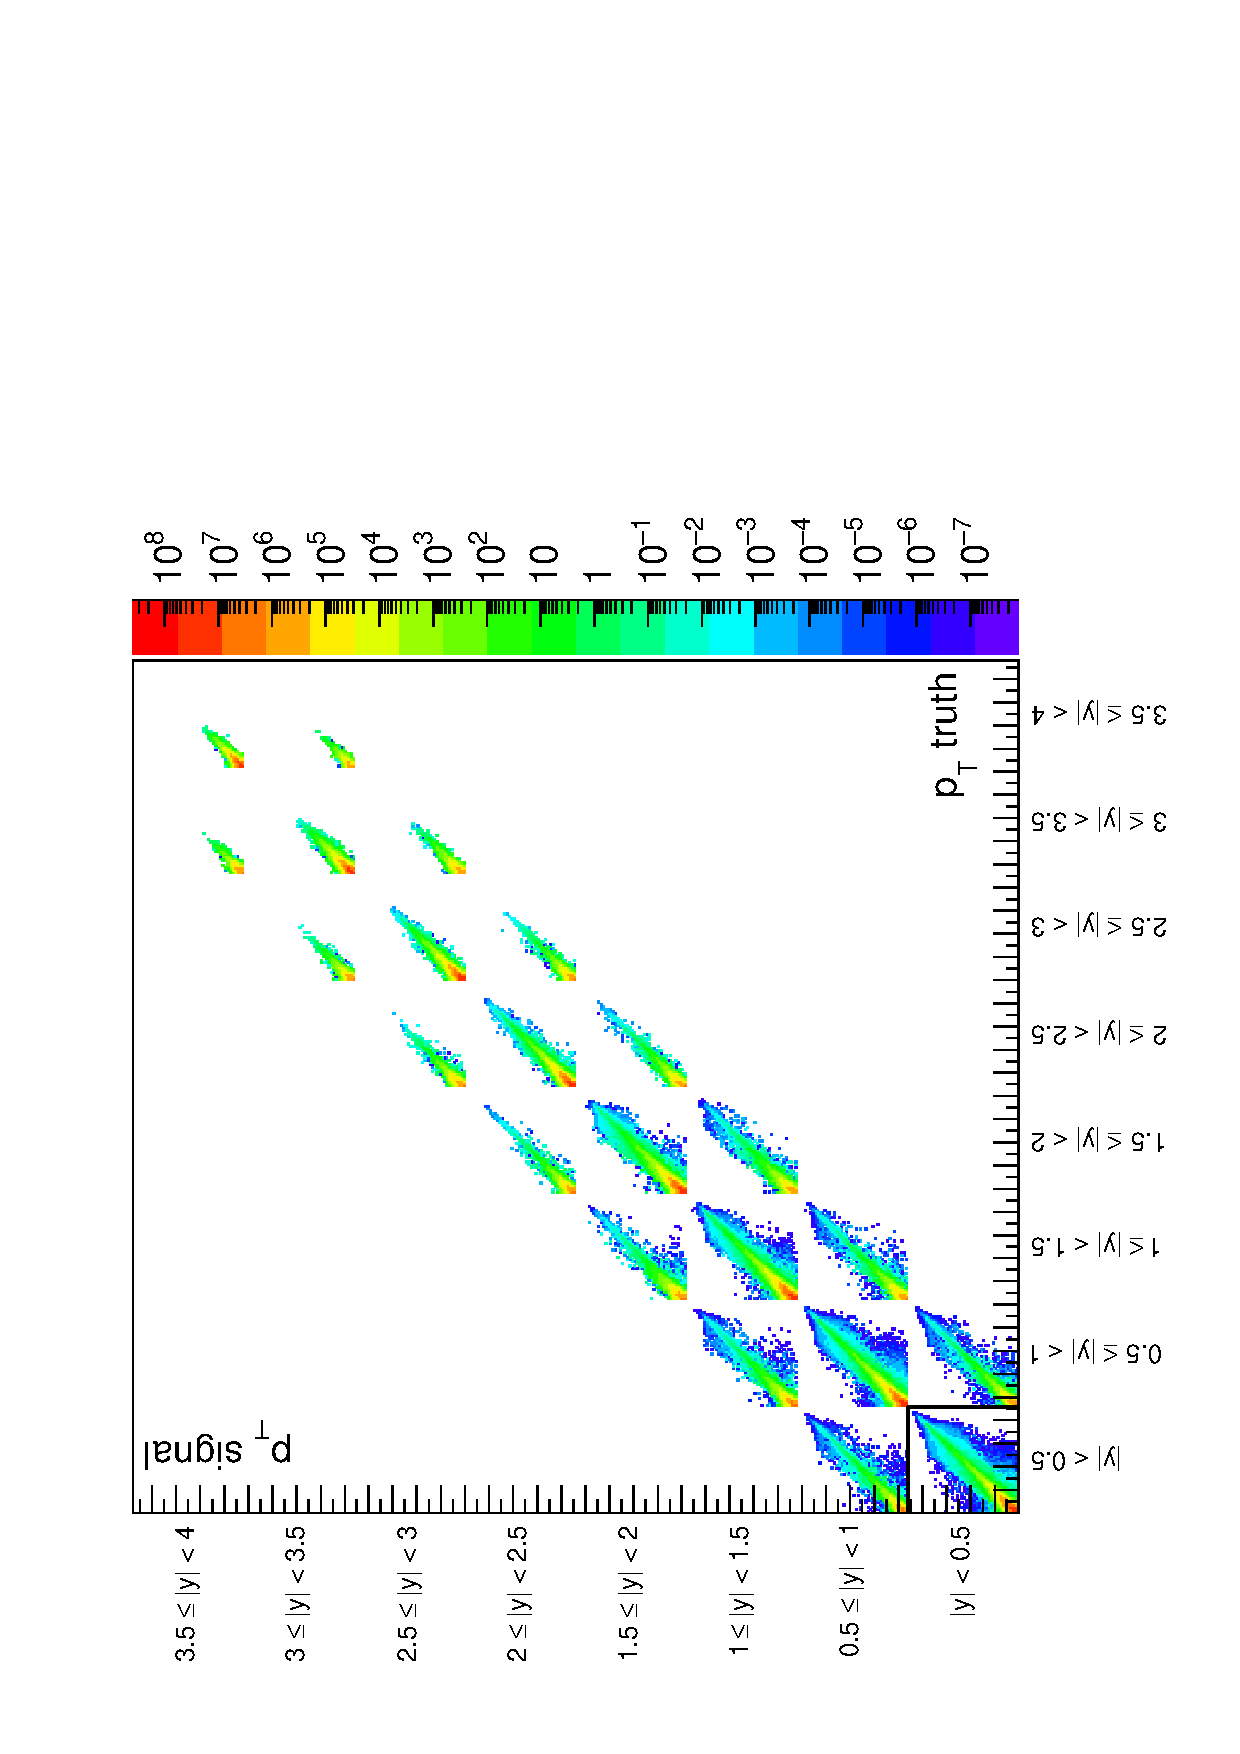
\includegraphics[width=\textwidth]{{Chapter3/Unfold_matrix_all}.eps}
  \caption{Unfolding matrix all}
  \label{fig:UnfoldingMatrixAll}
\end{figure}

\begin{figure}[p]
  \centering
  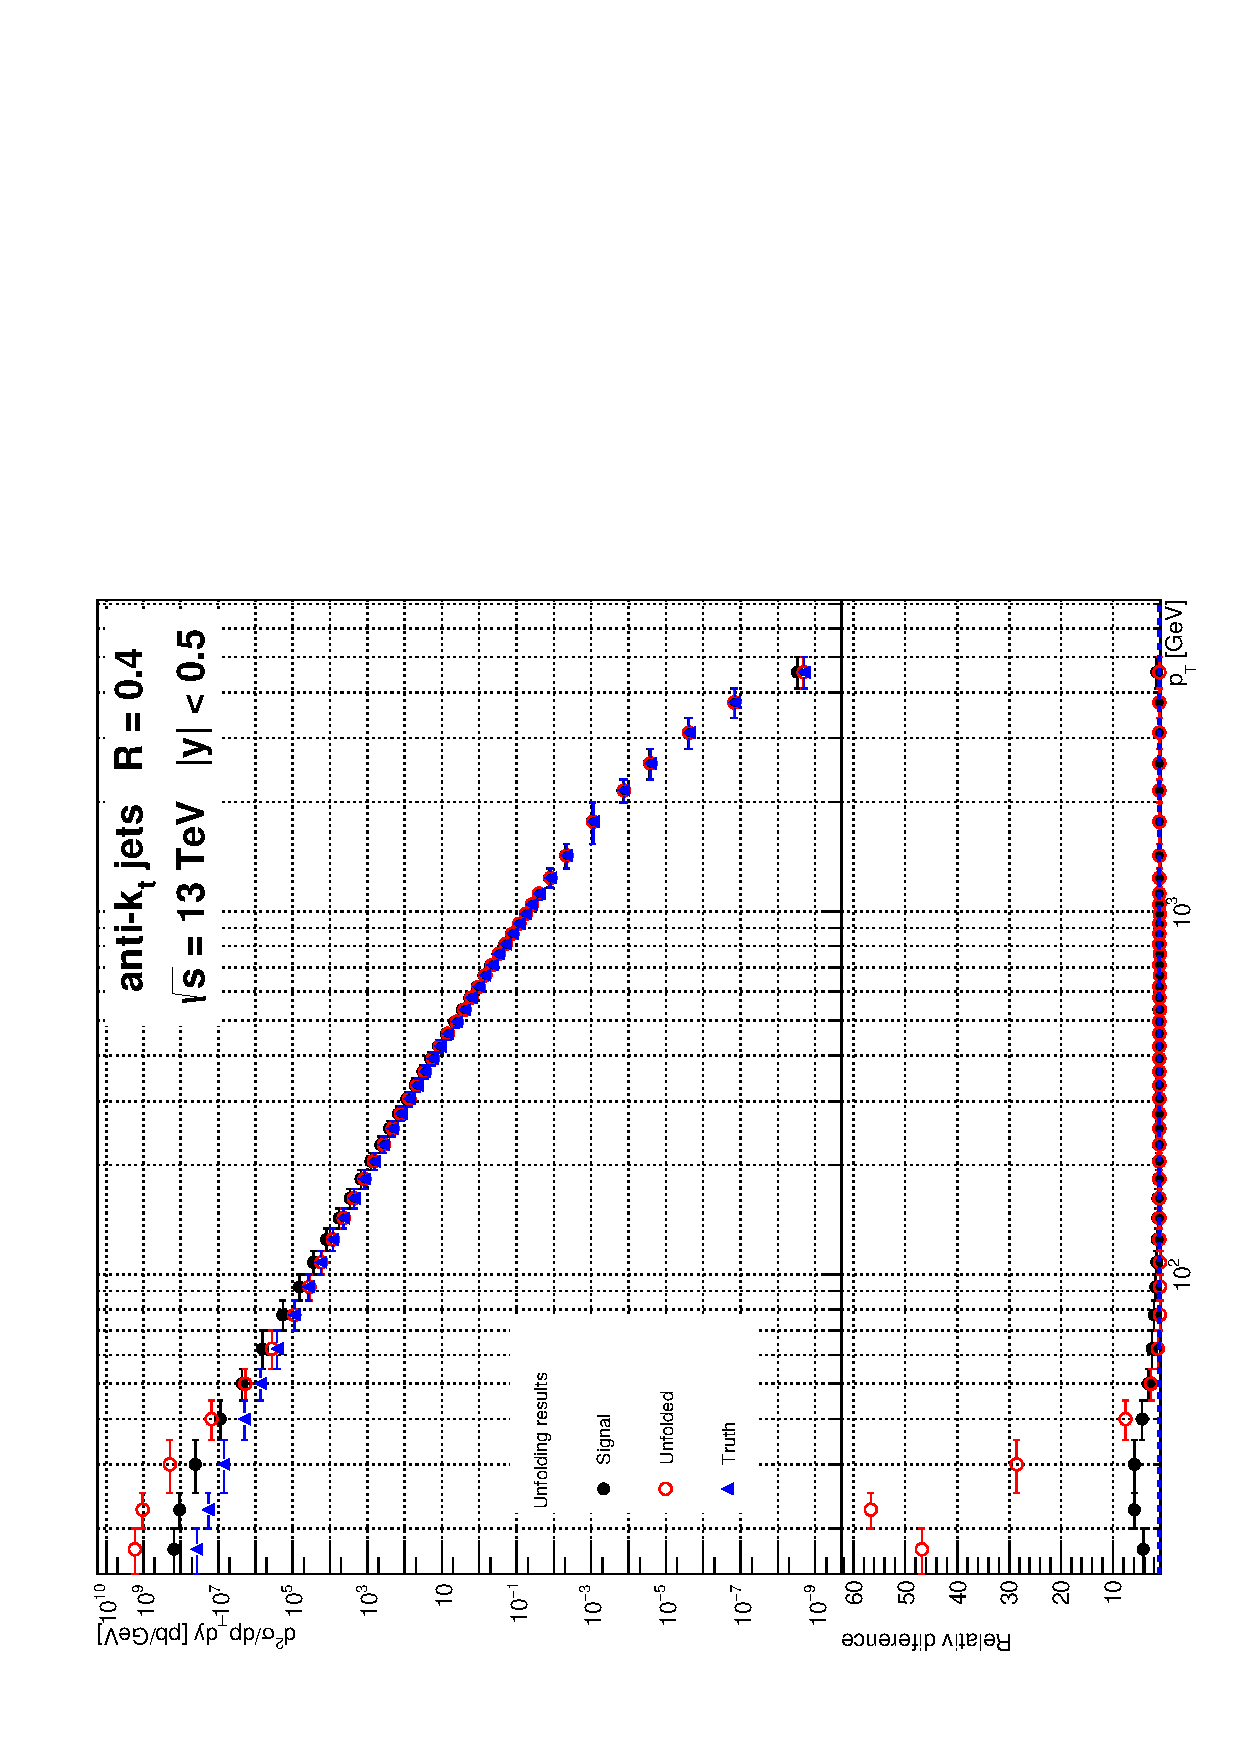
\includegraphics[width=\textwidth]{{Chapter3/Signal_VS_Unfold_VS_Truth_abs(y)0-0.5}.eps}
  \caption{Unfolding0}
  \label{fig:Unfolding0}
\end{figure}


\section{Comparison with Prediction}

\begin{figure}[p]
  \centering
  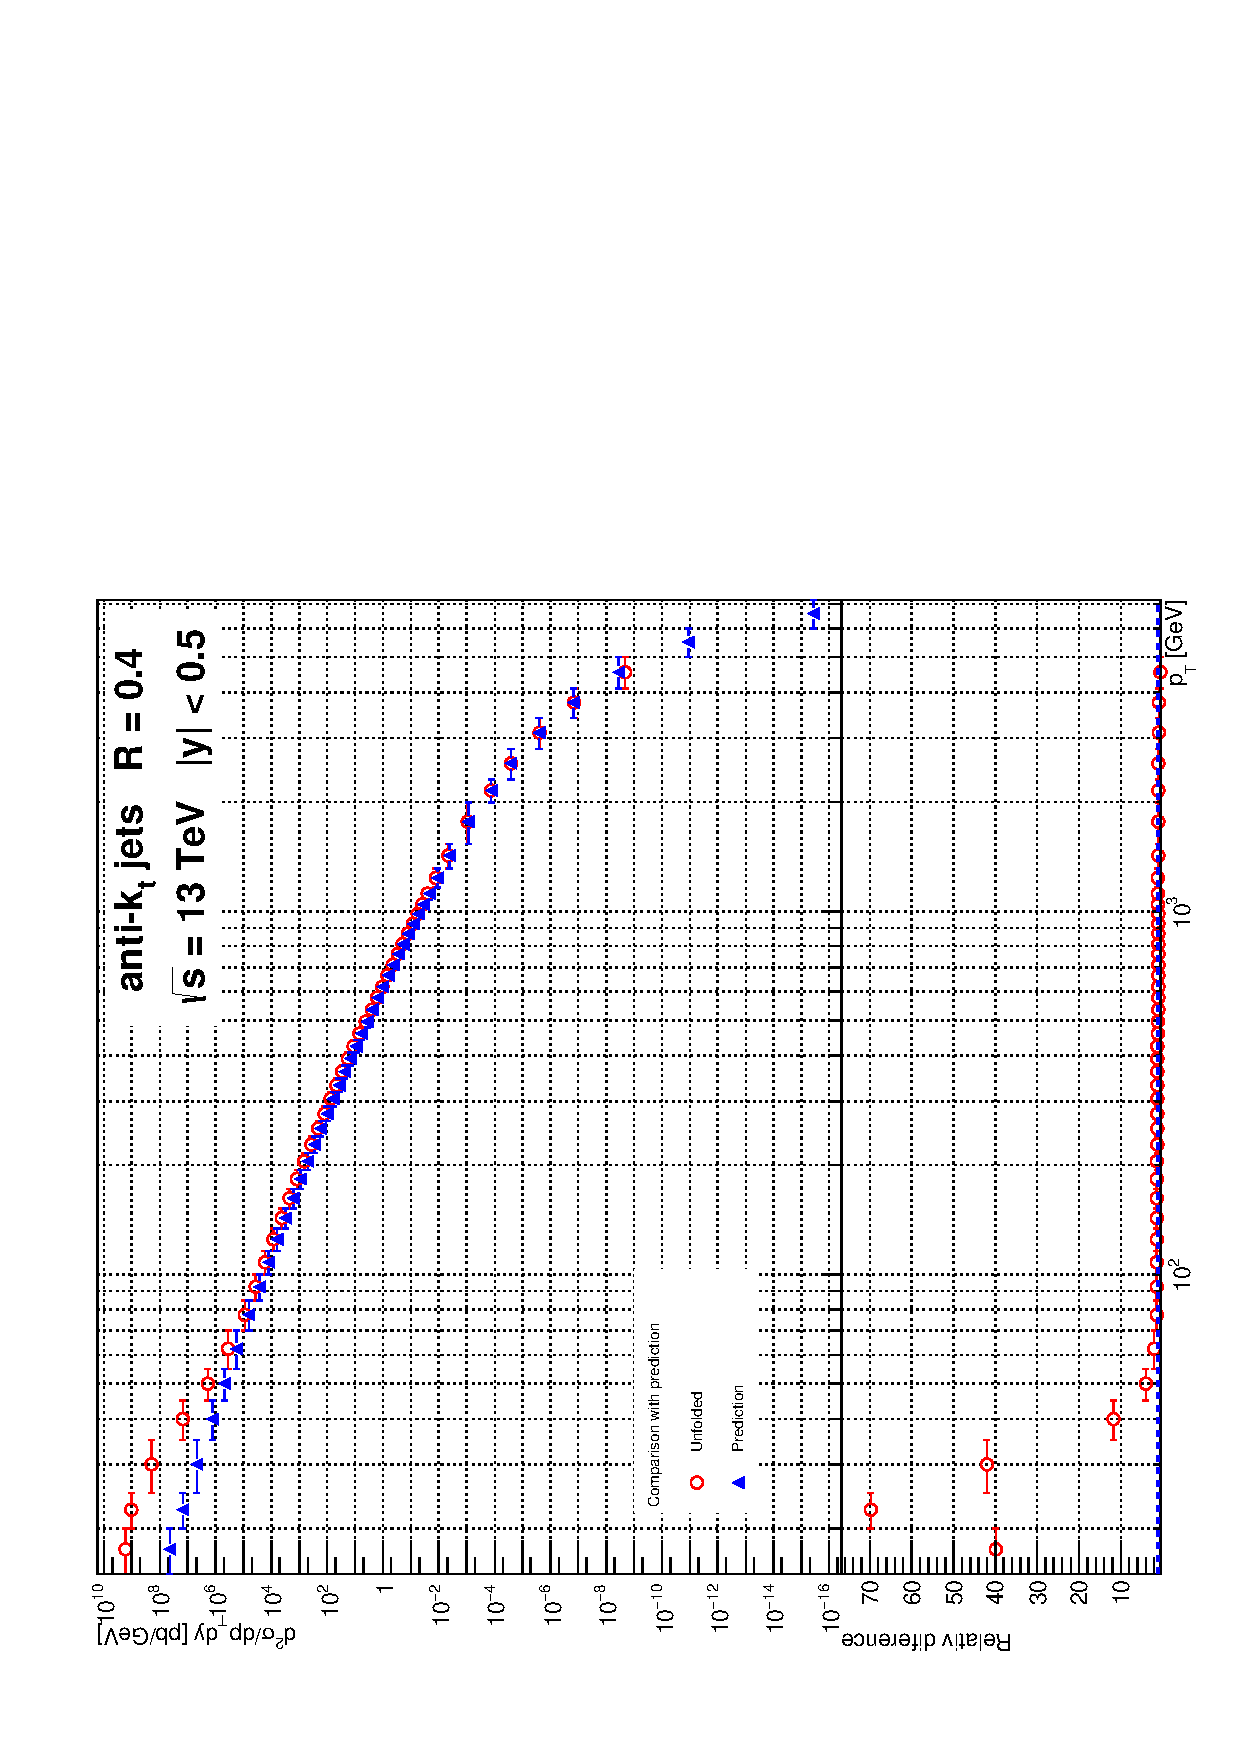
\includegraphics[width=\textwidth]{{Chapter3/Unfolded_VS_Prediciton_abs(y)0-0.5}.eps}
  \caption{Comparision unfolding with prediction 0}
  \label{fig:CompareUnfoldPred0}
\end{figure}
